\documentclass[a4paper, 12pt]{article}
%\documentclass[12pt]{book}    % For the book class

\usepackage[utf8]{inputenc}
\usepackage{kotex}
\usepackage{titlesec}
\usepackage{geometry}
\usepackage{fancyhdr}
\usepackage{afterpage}
\usepackage{graphicx}
\usepackage{caption}
%\usepackage{natbib}
\usepackage[numbers]{natbib}
\usepackage{mathptmx}
\usepackage{tocloft}
\usepackage{tabularx}
\usepackage{setspace}
\usepackage{algorithm}
\usepackage{algorithmicx}
\usepackage{algpseudocode}
\usepackage{listings}
\usepackage{color} % for custom colors
\usepackage{indentfirst}
\usepackage{amsmath, amssymb}
\usepackage{float} 
\usepackage{breakcites}
\usepackage{setspace}
\usepackage{hyperref}
\usepackage{setspace}
\usepackage{appendix}



% Define Python code style
\lstdefinestyle{pythoncode}{
  language=Python,
  backgroundcolor=\color{lightgray},
  commentstyle=\color{green},
  keywordstyle=\color{blue},
  numberstyle=\tiny\color{gray},
  stringstyle=\color{red},
  basicstyle=\ttfamily\small,
  breaklines=true,
  frame=single,
}

% 페이지 설정
\geometry{top=35mm, bottom=30mm, left=30mm, right=30mm, headheight=15mm, footskip=15mm}

% 섹션 스타일 설정
\titleformat{\section}{\fontsize{16pt}{19pt}\selectfont\bfseries}{\thesection}{1em}{}
\titleformat{\subsection}{\fontsize{14pt}{17pt}\selectfont\bfseries}{\thesubsection}{1em}{}
\titleformat{\subsubsection}{\fontsize{12pt}{14pt}\selectfont}{\thesubsubsection}{1em}{}
\titleformat{\subsubsubsection}{\fontsize{12pt}{14pt}\selectfont}{\thesubsubsection}{1em}{}

\renewcommand{\thesection}{\arabic{section}}

% 표와 그림의 캡션 스타일 설정
%\captionsetup{font={size=12pt, bf},labelfont={size=12pt, bf},labelsep=period}

% 헤더 & 푸터 설정
\fancyhf{}
%\pagestyle{fancy}

% ToC custom settings for sections
\renewcommand{\cftsecfont}{\fontsize{16pt}{19pt}\selectfont\bfseries}


% ToC custom settings for subsections and subsubsections
\renewcommand{\cftsubsecfont}{\fontsize{14pt}{17pt}\selectfont\bfseries}
\renewcommand{\cftsubsubsecfont}{\fontsize{12pt}{14pt}\selectfont}

% ToC vertical spacing settings
\setlength{\cftbeforesecskip}{10pt}
\setlength{\cftbeforesubsecskip}{5pt}
\setlength{\cftbeforesubsubsecskip}{5pt}
\cfoot{\thepage}


% 인용 형식
\setstretch{1.25} % 1.25배 줄 간격


\begin{document}
\setlength{\parindent}{1em} % 1em 대신 원하는 크기로 설정

% 논문요약 페이지
\begin{flushright}
    \rule{16cm}{5pt}\vskip1cm
    \begin{bfseries}
        \Huge{SOFTWARE REQUIREMENTS\\ SPECIFICATION}\\
        \vspace{1.9cm}
        for\\
        \vspace{1.9cm}
        SKKU PPT\\
        \vspace{1.9cm}
        \large{Version 1.0 approved}\\
        \vspace{1.9cm}
        Prepared by Team 13:
        
        \vspace{1.9cm}
        Sungkyunkwan University\\
        \vspace{1.9cm}
        \today \\
    \end{bfseries}
\end{flushright}
\newpage

\tableofcontents

\newpage


\begin{table}[H]
\centering
\begin{tabularx}{\textwidth}{|l|l|X|l|}
\hline
\textbf{Name} & \textbf{Date} & \textbf{Reason for Changes} & \textbf{Version} \\
\hline
Yosep Kim & 2023-11-05 & Initial document creation & 1.0 \\
\hline
\end{tabularx}
\caption{Document Revision History}
\label{table:revision_history}
\end{table}


\newpage


\section{Introduction}
\subsection{Purpose}

본 문서는 SKKUPPT 프로젝트의 근간을 이루는 다양한 요소들에 대해 심층적으로 서술하며, 그 목적은 프로젝트 참여자들에게 명확한 지침과 참조 자료를 제공함으로써, 일관된 이해와 효율적인 개발 과정을 돕는 데 있다. 이를 통해 프로젝트 팀은 사용자 중심의 디자인, 직관적인 기능 구현, 그리고 최적화된 사용자 경험을 목표로 SKKUPPT를 개발할 수 있다. 본 문서는 다음 세 가지 주요 세부 요구사항을 포함하며, 각각에 대해 구체적인 설명과 지침을 제공한다.

\begin{enumerate}
\item \textbf{하드웨어 및 소프트웨어 인터페이스:} 이 섹션에서는 SKKUPPT가 어떻게 다양한 하드웨어 장치들과 상호작용하며, 어떤 소프트웨어 인터페이스를 필요로 하는지 상세히 설명한다. 애플리케이션의 효율적인 작동을 위해 필요한 최소 사양, 호환 가능한 운영 체제, 그리고 외부 시스템이나 서비스들과의 통합 방법 등이 이에 포함된다.

\item \textbf{기능적 요구사항:} 사용자가 SKKUPPT를 통해 달성하고자 하는 목표를 실현하기 위해 애플리케이션은 다양한 기능들을 제공해야 한다. 이 섹션에서는 사용자가 어떤 작업을 수행할 수 있는지, 그리고 그 작업들이 어떻게 이루어지는지에 대한 자세한 정보를 제공한다. 각 기능은 명확한 시나리오, 기대되는 결과, 그리고 예외 처리 방안들을 포함하여 상세하게 기술될 것이다.

\item \textbf{비기능적 요구사항:} 애플리케이션의 성공적인 운영에 있어 기능적 측면만큼 중요한 것이 비기능적 측면이다. 이 섹션은 시스템의 성능 기준, 안정성, 사용 가능성, 그리고 보안을 포함한 품질 요구사항들을 다룬다. 여기에는 응답 시간, 동시 사용자 수, 데이터 보호 정책, 백업 절차 등 시스템이 충족해야 할 표준과 프로토콜에 대한 상세한 기준이 포함된다.
\end{enumerate}

이러한 요구사항들은 프로젝트의 성공적인 완성을 위한 토대를 마련하고, 개발자와 이해관계자 모두가 동일한 비전을 공유하며 협업할 수 있는 환경을 조성하는 데 중요한 역할을 한다.



\subsection{Document Conventions}
본 문서 내에서 사용되는 용어와 정의는 이해를 돕기 위해 일관된 규약에 따라 제시되었다. 아래에 제시된 표는 본 문서와 SKKUPPT 프로젝트 전반에 걸쳐 일관되게 사용될 주요 용어들과 그에 대한 설명을 정리한 것이다. 이 표를 참조함으로써, 독자들은 프로젝트에 관련된 기술적 표현과 용어의 정확한 의미를 파악할 수 있으며, 개발 과정 및 문서에 대한 이해도를 높일 수 있다.

\subsubsection{Definitions and Terminologies}
\begin{table}[H]
\centering
\begin{tabularx}{\textwidth}{|c|X|}
\hline
\textbf{용어} & \textbf{설명} \\
\hline
유저 & PPT 구조 자동 생성 프롬프트 SKKUPPT의 사용하는 모든 유저 \\
\hline
관리자 & SKKUPPT의 기능 및 데이터베이스를 관리하고 제작하는 사람 \\
\hline
백엔드 & 소프트웨어 개발 프로세스 중 DB 같은 서버 사이드 부분 \\
\hline
프론트엔드 & 백엔드에서 가져온 데이터의 출력, 입력을 통한 로직 구성과 사용자와 대화하는 사용자 인터페이스 부분 \\
\hline
웹 & 인터넷에 연결된 컴퓨터를 통해 사람들이 정보를 공유할 수 있는 전 세계적인 정보 공간 \\
\hline
IT 인프라 & 네트워크, 서버, 데이터베이스, 정보보안, 시스템 소프트웨어 및 기반시설 등 IT서비스의 기반이 되는 시스템 및 구조 \\
\hline
\end{tabularx}
\caption{본 연구에서 강조하는 주요 용어 및 설명}
\label{table:definition}
\end{table}

이 표는 문서 내용의 일관성과 명확성을 위해 설정된 용어 사용 기준을 제공한다. 예를 들어, '사용자'는 SKKUPPT의 애플리케이션 사용자를 의미하며, '관리자'는 시스템을 관리하고 제작하는 사람을 지칭한다. 표에 명시된 '백엔드'와 '프론트엔드'는 각각 애플리케이션의 서버 사이드 및 클라이언트 사이드 개발에 관련된 용어로 사용되며, 이는 개발 과정에서 중요한 구분이다. '웹'은 인터넷을 기반으로 한 전반적인 정보 공간을 나타내며, 'IT 인프라'는 이러한 서비스들을 지원하는 기본적인 기술적 구조를 의미한다.

본 용어 정의 표는 문서 내 모든 관련 용어에 대한 참조 지침으로 활용될 것이며, 이를 통해 효과적인 의사소통과 프로젝트의 원활한 진행을 지원한다.

\subsubsection{Abbreviations and Acronyms}

본 문서 및 SKKUPPT 프로젝트의 커뮤니케이션에서 일반적으로 사용되는 약어와 약칭은 의사소통을 간소화하고 문서의 간결성을 유지하기 위해 사용된다. 아래 표는 프로젝트 관련 문서와 토론에서 자주 등장하는 기술 용어의 약어를 나열하며, 각각의 전체 용어를 설명한다. 이러한 약어의 정의는 모든 참여자가 용어에 대한 일관된 이해를 가지고 의사소통할 수 있도록 함으로써, 혼란을 최소화하고 프로젝트의 효율성을 높이는 데 기여한다.

\begin{table}[H]
\centering
\begin{tabularx}{\textwidth}{|l|X|}
\hline
\textbf{약어} & \textbf{설명} \\
\hline
UI & User Interface \\
\hline
App, 앱 & Application \\
\hline
DB & Database \\
\hline
API & Application Programming Interface \\
\hline
AWS EC2 & Amazon Web Services Elastic Compute Cloud \\
\hline
OS & Operating System \\
\hline
FE & Front End \\
\hline
BE & Back End \\
\hline
LLM & Large Language Model \\
\hline
\end{tabularx}
\caption{주요 약어 및 설명}
\label{table:abbreviations}
\end{table}



이 표를 통해 독자들은 UI, DB, API 등의 약어가 각각 사용자 인터페이스, 데이터베이스, 응용 프로그래밍 인터페이스를 의미하는 것을 쉽게 이해할 수 있다. 특히 AWS EC2와 같은 약어는 특정 기술이나 서비스를 지칭할 때 그 의미가 명확해져, 텍스트를 읽거나 작성할 때 시간을 절약할 수 있다. FE와 BE는 각각 프론트 엔드와 백 엔드를 가리키며, 이는 개발의 두 주요 영역을 나타낸다. LLM은 본 문서에서 중요한 개념인 '대형 언어 모델'을 의미하며, 이는 GPT와 같은 인공 지능 시스템을 지칭할 때 사용된다.


\subsection{Intended Audience and Reading Suggestions}
본 문서의 타깃 독자는 SKKUPPT 애플리케이션의 개발자인 13조 구성원과 이를 사용할 주된 이용자인 성균관대학교 교수, 학생 및 조교들이다. 문서 작성 과정에서는 IEEE의 표준적인 SRS 규격 \cite{ieee830}을 준수하였으며, 관련 우수 사례들 \cite{parkingo}\cite{skkunare}도 참고하였다.

본 소프트웨어 요구 사양(Software Requirement Specification, SRS) 문서는 소프트웨어의 기능과 제약 사항, 그리고 개발에 필요한 사항들을 명시하고 있다. 이 문서는 총 5개의 주요 장(Chapter)과 참조문헌(References), 그리고 세 개의 부록(Appendix)으로 구성되어 있으며, 이를 통해 SKKUPPT 애플리케이션의 구조와 요구사항을 명확히 제시한다.

\begin{itemize}
\item \textbf{제1장 도입(Introduction)}: 이 장에서는 문서의 목적과 범위, 사용된 약어 및 용어에 대한 설명이 포함된다. 또한 소프트웨어의 개요 및 본 문서가 적용하는 기준과 관례에 대해서도 언급한다.

\item \textbf{제2장 전체 설명(Overall Description)}: 제품의 관점, 기능, 사용자 클래스 및 특성, 운영 환경, 설계 및 구현상의 제약조건, 사용자 문서화, 가정 및 의존성 등을 다룬다. 이 장은 시스템이 어떻게 운영될지에 대한 큰 그림을 제공한다.

\item \textbf{제3장 외부 인터페이스 요구사항(External Interface Requirements)}: 사용자, 하드웨어, 소프트웨어, 통신 인터페이스에 대한 상세한 설명이 포함된다.

\item \textbf{제4장 시스템 기능(System Features)}: 사용자 인증, 서비스 선택, PPT 메이커 등 주요 기능에 대한 설명 및 우선 순위, 자극/응답 순서, 기능적 요구사항을 자세히 기술한다.

\item \textbf{제5장 비기능적 요구사항(Non-Functional Requirements)}: 성능, 안전, 보안 요구사항과 소프트웨어 품질 속성 및 비즈니스 규칙 등에 대해 설명한다.
\end{itemize}
\subsection{Product Scope}
본 문서는 성균관대학교 소프트웨어 공학개론 수업의 13조 학생들이 개발할 SKKUPPT 애플리케이션에 대한 시스템 및 사용자 요구사항을 명시한다. SKKUPPT의 Product Scope은 다음과 같다. 

\begin{itemize}
  \item \textbf{자동화된 PPT 구조 생성:} 사용자가 주제와 방향만 제공하면, SKKUPPT는 자동으로 해당 내용에 적합한 PPT 레이아웃을 생성한다. 이 기능은 사용자가 과제의 본질에 보다 집중할 수 있게 돕는다.
  \item \textbf{시간 및 노력 절약:} PPT 레이아웃 및 디자인 결정에 소요되는 시간과 노력을 줄여, 사용자는 보고서의 내용에 더 많은 시간을 할애할 수 있다.
  \item \textbf{품질 향상:} 자동화된 서비스를 통해 사용자는 프레젠테이션의 전반적인 품질을 향상시킬 수 있다.
\end{itemize}


%\subsection{References}
\begin{spacing}{1.25} % Adjust the spacing here. 1.25 is one-and-a-quarter spacing, you can adjust as needed.
\phantomsection % This ensures correct destination of the hyperlink
\addcontentsline{toc}{subsection}{References}
\renewcommand\bibname{References} % Rename "Bibliography" to "References"
\bibliographystyle{IEEEtran}
\bibliography{references}
\end{spacing}

\section{Overall Description}
\subsection{Product Perspective}
SKKUPPT는 성균관대학교 학생들을 위한 GPT 기반 PPT 슬라이드 자동 제작 웹 애플리케이션입니다. SKKUPPT는 사용자가 입력한 프롬프트와 소스에 따라 완성된 PPT 파일을 제공함으로써 학생들이 프레젠테이션 및 과제에 드는 시간을 절감하여 학습에 집중할 수 있도록 합니다.
\subsubsection{System Interfaces}
사용자의 계정에 대한 모든 데이터와 PPT 슬라이드 제작 데이터는 서버에 저장됩니다. 데이터베이스는 AWS EC2 인스턴스 내에서 호스팅 되며, 데이터베이스 엔진 (ex: MySQL, PostgreSQL, MongoDB 등)에 따라 구성됩니다. 모든 요청 및 응답 데이터는 RESTful API 형태로 구현되며, HTTP, TCP, IP 프로토콜과 JSON 포맷을 따릅니다.
\subsubsection{User Interfaces}
사용자 인터페이스는 모바일 및 데스크톱 디바이스의 웹 브라우저를 통해 접근 가능하며, 사용하는 기기의 입력 장치를 통해 데이터를 입력 받습니다. 

사용자는 새 슬라이드 생성을 통해 신규 PPT 슬라이드를 생성할 수 있고, 디자인한 PPT 슬라이드를 확인 및 수정할 수 있습니다. 또한 신규 슬라이드 작성 시 템플릿을 선택하여 상황에 맞는 디자인을 적용할 수 있습니다.

\subsection{Product Functions}
\subsubsection{Sign-in and Sign-up}
모든 사용자는 웹 페이지 접근 시, 이메일과 비밀번호 입력 후 로그인이 가능합니다. 미등록 사용자는 회원가입을 통해 사용 등록이 가능하며, 회원가입에는 이메일 입력과 이메일 인증을 위한 인증번호 입력, 비밀번호 설정 과정이 필요합니다. 또한 구글 계정과 연동하여 회원가입을 하지 않고 로그인이 가능합니다.

\subsubsection{Write Prompt}
사용자는 프롬프트 작성 과정을 통해 각 슬라이드에 사용될 템플릿을 설정하고 내용과 소스를 입력하여 구성할 수 있습니다. 프롬프트 작성은 자연어로 구성되며 지시 사항이 구체적일수록 더 디테일한 결과를 얻을 수 있습니다. 들어갈 수 있는 소스에는 이미지 파일, 텍스트가 있습니다.

\subsubsection{Create PPT Slide}
사용자가 프롬프트 작성을 마치면 프로그램은 PPT 슬라이드 구성을 디자인하고, 내용을 작성하여 완성된 파일을 제공합니다. 해당 파일은 웹 페이지의 다운로드 버튼을 눌러 사용자가 지정한 형식 및 위치에 저장할 수 있습니다.

\subsubsection{Identify User Trends}
사용자의 PPT 슬라이드 입력 및 생성된 슬라이드에 대한 데이터를 수집하고 저장합니다. 저장되는 데이터에는 사용자의 디자인 선호도, 텍스트 스타일을 포함합니다.

해당 프로그램은 기계 학습 알고리즘을 사용하여 사용자 데이터를 분석하고 이를 기반으로 PPT 슬라이드의 스타일 및 어투를 최적화하여 다음 PPT 슬라이드 생성에 반영합니다.
\subsection{User Classes and Characteristics}
해당 애플리케이션에서 사용자는 PPT 슬라이드 제작자를 지칭합니다. PPT 슬라이드 제작자는 한국어 또는 영어를 사용할 수 있는 능력이 있고, PPT 슬라이드를 제작 시 필요한 프로그램 도구들을 사용할 수 있다고 가정합니다.
\subsection{Operating Environment}

웹 애플리케이션의 원활한 운영을 보장하기 위해서는 하드웨어와 소프트웨어 구성 요소를 포함한 운영 환경을 고려하는 것이 중요합니다. 기본 기능성과 성능을 보장하기 위한 최소 요구 사항은 아래에 명시되어 있습니다.

\subsubsection{Hardware}
\paragraph{프로세서}
해당 웹 애플리케이션은 적어도 1GHz 단일 코어 프로세서를 필요로 합니다. 이는 웹 애플리케이션의 작업을 상당한 지연 없이 처리할 수 있는 기본 처리 능력을 보장합니다.

\paragraph{메모리}
웹 애플리케이션을 위해서는 최소 1GB의 RAM이 필요합니다. 충분한 메모리는 멀티태스킹을 위해 중요하며, 웹 애플리케이션의 원활한 실행을 보장하는 데 필수적입니다.

\paragraph{저장 공간}
웹 애플리케이션 자체가 상당한 저장 공간을 필요로 하지는 않지만, 적어도 100MB의 여유 공간을 갖는 것이 좋습니다. 이는 임시 파일과 캐시를 저장할 수 있도록 하여 전반적인 성능에 영향을 주지 않습니다.

\paragraph{네트워크}
웹 애플리케이션에 접속하기 위해서는 안정적인 인터넷 연결이 요구됩니다. 반응형 사용자 경험을 유지하기 위해 최소한 1Mbps 다운로드 속도의 광대역 연결을 권장합니다.

\subsubsection{Software}
\paragraph{운영체제}
웹 애플리케이션은 다양한 운영체제와 호환되도록 설계되었습니다. 윈도우 사용자의 경우, 최신 보안 기능과 업데이트를 활용하기 위해 윈도우 10 이상의 버전이 요구됩니다.

\paragraph{웹 브라우저}
적어도 하나의 현대적인 웹 브라우저가 설치되어 있어야 합니다. 웹 애플리케이션은 Mozilla Firefox, Google Chrome, Apple Safari 등의 최신 버전 브라우저와 호환됩니다. 웹 브라우저를 최신 상태로 유지하는 것은 호환성 문제를 피하고 웹 애플리케이션의 보안을 보장하는 데 중요합니다.

\paragraph{지원 소프트웨어}
웹 애플리케이션의 특정 기능은 Adobe Reader, Java 또는 특정 플러그인과 같은 추가 소프트웨어를 필요로 할 수 있습니다. 사용자는 웹 애플리케이션의 문서를 확인하여 추가 소프트웨어 요구 사항을 확인하고 필요에 따라 설치해야 합니다.

\subsection{Design and Implementation Constraints}
본 어플리케이션은 철저한 시장 조사와 사용자 피드백을 기반으로 한 세심한 설계 철학을 바탕으로 개발될 예정이다. 이를 위해 다음과 같은 다양한 세부 체크리스트를 엄격히 준수한다.

\begin{itemize}
  \item 사용자 중심 설계: 사용자의 최적의 편의성을 제공하고, 다양한 요구사항을 만족시키기 위한 유연한 확장성과 뛰어난 가용성을 고려한 개발 전략을 채택한다.
  \item 비용 효율성: 오픈소스 소프트웨어의 적극적인 활용을 통해 개발 비용을 절감하며, 사용자에게 비용 부담 없는 서비스를 제공한다.
  \item 직관적인 UI 설계: 최첨단 사용자 경험 설계 원칙에 입각하여, 사용자에게 친숙하고 직관적인 인터페이스를 제공한다.
  \item 기술 통합: Chat GPT API와 같은 고급 기술을 통합하여, 인공 지능 기반의 혁신적인 기능을 제공한다.
  \item 다국어 지원: 글로벌 사용자 기반을 고려하여 한국어와 영어 지원을 포함한 다양한 언어 옵션을 제공한다.
  \item 최신 기술 스택 채택: Next.js, nginx, 클라우드 서비스 등의 현대적인 기술을 활용하여 강력하고 확장 가능한 애플리케이션을 개발한다.
  \item 최적화된 성능: 리소스 낭비를 방지하고 최적화된 소스 코드를 통해 빠르고 효율적인 서비스를 구현한다.
  \item 광범위한 호환성: Microsoft Edge, Firefox, Chrome, Opera, Safari 등 주요 웹 브라우저와 Windows, Linux, MacOS 등의 주요 운영체제에서 무리 없는 실행을 보장한다.
  \item 표준화된 통신 프로토콜: HTTP 프로토콜을 기반으로 안정적이고 보안성 높은 사용자 디바이스와 서버 간 통신을 구현한다.
\end{itemize}

\subsection{User Documentation}
사용자가 어플리케이션을 최대한 활용할 수 있도록 광범위한 지원 문서를 제공한다. 다음은 사용자 문서화를 위한 포괄적인 가이드라인이다.

\begin{enumerate}
  \item 시스템 요구사항 문서: 사용자가 어플리케이션을 원활하게 사용하기 위한 하드웨어 및 소프트웨어 요구사항에 대한 상세한 정보를 제공한다.
  \item 사용자 매뉴얼: 어플리케이션이 어떠한 목적으로 개발되었는지, 사용자가 입력해야 할 데이터의 형식, 기대할 수 있는 결과물의 다양한 형태를 포함한 상세한 지침서를 제공한다. 또한 입력 값과 예상 결과 사이의 관계를 명확히 하는 스크린샷을 포함시켜 사용자의 이해를 돕는다.
  \item 개발자 연락처: 사용자가 문제를 보고하거나 피드백을 제공할 수 있도록 어플리케이션 개발자의 연락 정보를 명시한다.
\end{enumerate}

\subsection{Assumptions and Dependencies}
본 어플리케이션은 Chrome, Firefox, Safari 등의 주요 웹 브라우저와 Windows, Mac, Android 등의 다양한 운영체제에서 원활히 작동됨을 가정한다. 이는 어플리케이션의 접근성을 극대화하고, 다양한 기기와 플랫폼에서의 이용 가능성을 확보한다는 의미이다. 따라서, 사용자가 웹 브라우저에 접속할 수 있는 어떠한 환경에서도 본 어플리케이션을 효과적으로 사용할 수 있을 것으로 예상한다.

\section{External Interface Requirements}

\subsection{User Interfaces Details}

\subsubsection{Registration User Interface}

새로운 사용자를 환영하고 서비스 생태계에 원활하게 통합하기 위해 등록 UI가 마련되어 있습니다.

\begin{itemize}
\item 사용자 신원을 설정하기 위해 유효한 이메일 주소를 입력하는 양식입니다.
\item 사용자 계정의 보안을 확보하기 위한 안전한 비밀번호 입력 필드입니다.
\item 완료시 즉시 새 사용자 계정을 인증하는 로그인 인터페이스로 전환됩니다.
\item 텍스트 필드의 명확성, 직관적인 레이아웃 및 사용자 입력 유효성에 대한 반응형 피드백을 포함한 디자인 고려 사항입니다.
\end{itemize}

Fig. \ref{fig:signup}은 사용자 등록 인터페이스를 보여줍니다.

\begin{figure}[H]
\centering
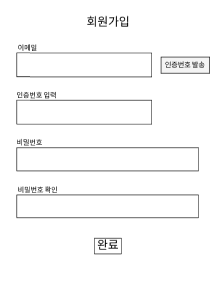
\includegraphics[width=0.4\textwidth]{img/signup.png}
\caption{회원 가입의 user interface}
\label{fig:signup}
\end{figure}

\subsubsection{Login User Interface}

로그인 UI는 반환 사용자가 시스템 내에서 개인 설정과 기록에 액세스할 수 있는 게이트웨이를 제공합니다.

\begin{itemize}
\item 사용자 계정에 액세스하기 위해 등록된 이메일과 해당 비밀번호를 입력하는 필드입니다.
\item 성공적인 로그인 시도는 사용자를 상호 작용을 위한 프롬프트 생성 인터페이스로 이동시킵니다.
\item 사용자가 로그아웃하기로 결정할 때까지 사용자 세션을 유지하는 시스템은 사용의 편의성과 사용 용이성을 향상시킵니다.
\item 사용자 정보를 보호하기 위해 입력된 데이터에 대한 암호화를 포함한 보안 조치가 구현되어 있습니다.
\end{itemize}

Fig. \ref{fig:login}은 로그인 사용자 인터페이스를 보여줍니다.

\begin{figure}[H]
\centering
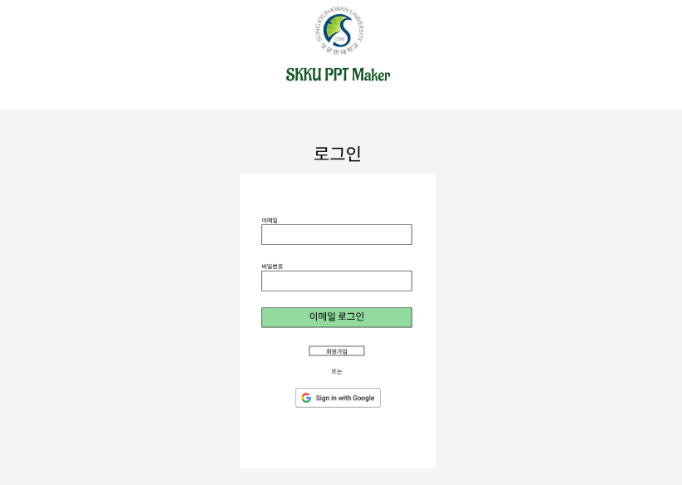
\includegraphics[width=1\textwidth]{img/login.png}
\caption{로그인 user interface}
\label{fig:login}
\end{figure}

\subsubsection{Prompt Creation User Interface}

이 UI는 사용자가 시스템이 출력을 생성하는 데 사용할 프롬프트를 만들 수 있도록 하는 서비스의 핵심 기능을 실현하는 곳입니다.

\begin{itemize}
\item 효과적인 프롬프트를 만들기 위한 제안과 개선 사항을 제공하는 동적 양식으로 주제, 테마, 말투 등의 정보를 입력하는 입력 필드입니다.
\item 제출 전에 사용자 입력을 편집하고 다듬을 수 있도록 프롬프트가 어떻게 구성되고 있는지 실시간 미리 보기를 제공합니다.
\item 사용자가 기대하는 입력 형식과 옵션을 이해하는 데 도움이 되는 시각적 단서와 도구 설명입니다.
\end{itemize}

Fig. \ref{fig:prompt}는 프롬프트 생성 사용자 인터페이스를 보여줍니다.

\begin{figure}[H]
\centering
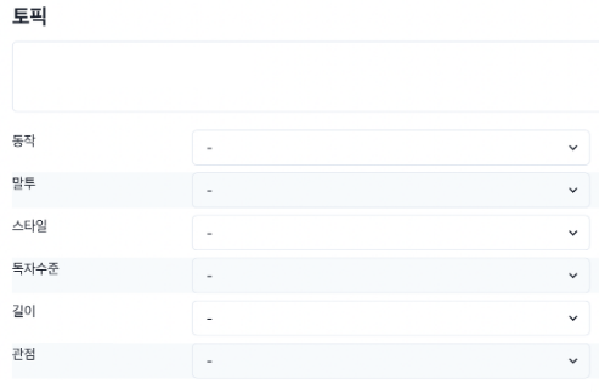
\includegraphics[width=1\textwidth]{img/prompt.png}
\caption{프롬프트 생성 user interfaces}
\label{fig:prompt}
\end{figure}

\subsubsection{Chat User Interface}

채팅 UI는 사용자가 챗봇 형식으로 GPT 생성 응답과 대화를 진행할 수 있는 대화형 플랫폼입니다.

\begin{itemize}
\item 대화 내역을 표시하는 대화 창으로 사용자가 대화를 따라갈 수 있도록 합니다.
\item 메시지 입력을 지원하고 멀티미디어 첨부 파일을 지원하는 입력 영역으로 커뮤니케이션 경험을 풍부하게 합니다.
\item 시스템의 응답으로부터 즉각적인 피드백을 제공하여 원활한 대화 흐름을 가능하게 합니다.
\item 새로운 사용자에게 친숙한 환경을 제공하기 위해 인기 있는 메시징 플랫폼을 모방한 디자인입니다.
\end{itemize}

Fig. \ref{fig:chat}은 채팅 사용자 인터페이스를 보여줍니다.

\begin{figure}[H]
\centering
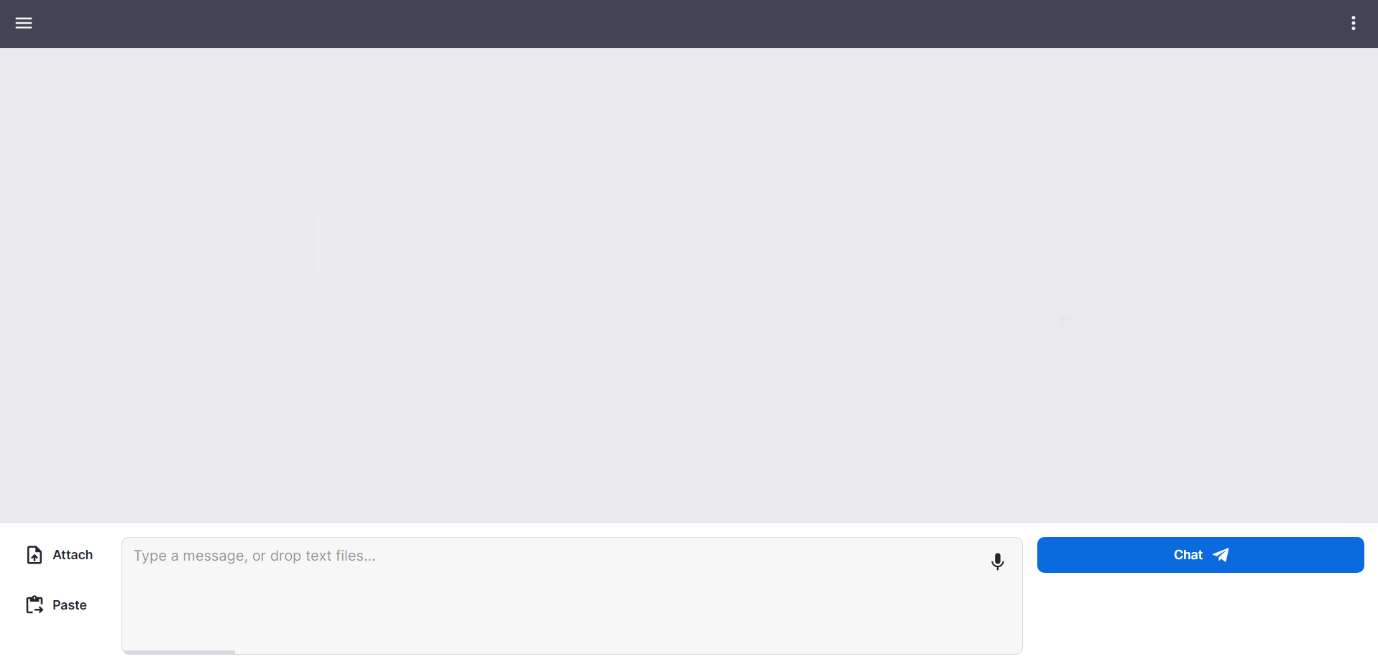
\includegraphics[width=1\textwidth]{img/chat.png}
\caption{채팅 User Interfaces}
\label{fig:chat}
\end{figure}

\subsubsection{Input User Interface}

입력 UI는 사용자가 추가 질의를 제공하고 피드백을 받을 수 있게 하여 시스템과의 양방향 커뮤니케이션 스트림을 가능하게 하는 중요한 기능입니다.

\begin{itemize}
\item 사용자가 질문, 제안 또는 명령을 입력할 수 있는 전용 공간입니다.
\item 사용자 입력에 기반한 시스템 피드백, 응답 및 프롬프트가 즉시 표시되어 상호 작용적이고 반복적인 프로세스를 가능하게 합니다.
\item 사용자가 응답을 평가하고 피드백을 제공할 수 있는 옵션으로 시스템의 학습과 시간이 지남에 따른 개선에 기여합니다.
\item 입력 제출, 지원 요청 또는 추가 시스템 리소스 접근을 위한 명확하고 접근하기 쉬운 옵션입니다.
\end{itemize}

Fig. \ref{fig:chat_input}는 입력 사용자 인터페이스를 보여줍니다.

\begin{figure}[H]
\centering
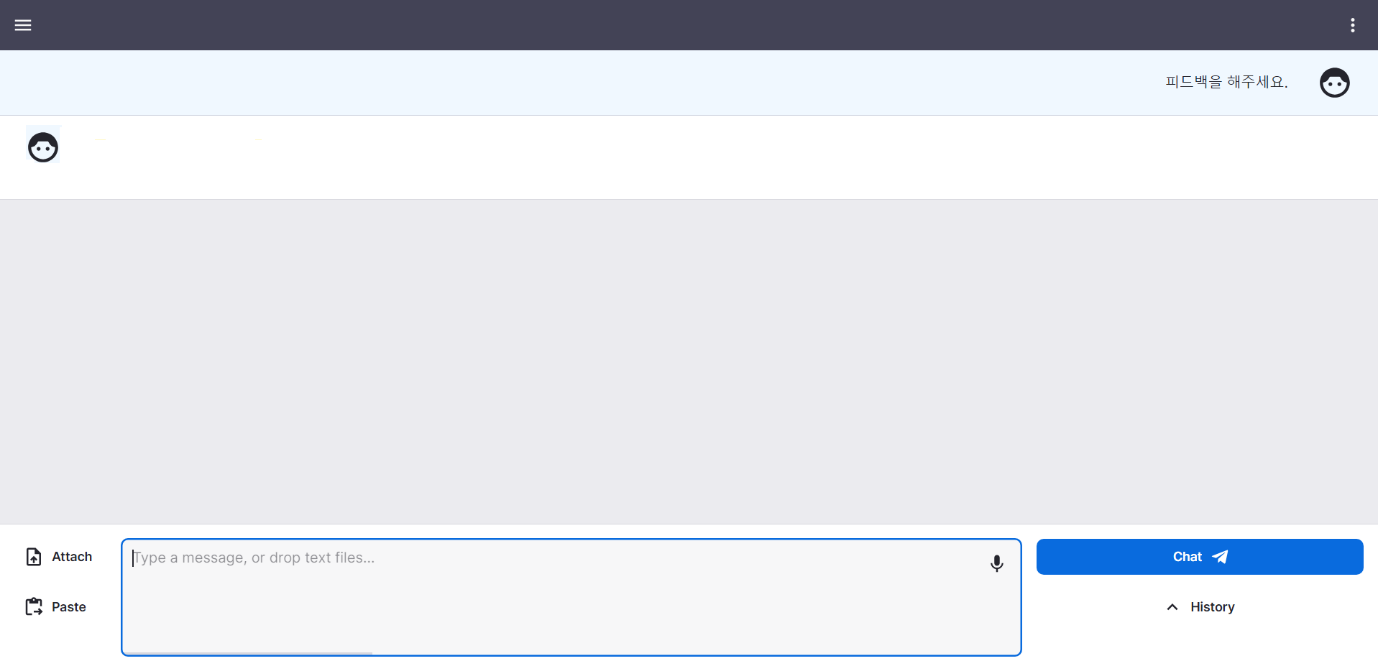
\includegraphics[width=1\textwidth]{img/chat_input.png}
\caption{입력 User Interfaces}
\label{fig:chat_input}
\end{figure}

각 인터페이스는 사용자 만족도를 극대화하기 위해 명확하고 간결하며 반응적인 사용자 경험을 제공하도록 설계되었으며, 사용자가 웹 서비스의 기능을 효율적으로 탐색하고 사용할 수 있도록 보장합니다.

\subsection{Hardware Interface}

시스템 접속을 위해서는 특정 하드웨어 사양이 요구됩니다. 이 사양에는 64비트 CPU, 최소 512MB의 RAM, 그리고 200MB 이상의 드라이브 공간이 포함되어 있어야 합니다. 사용자의 모바일 기기나 PC가 이러한 기준을 만족시켜야 시스템과의 호환성을 보장할 수 있습니다.

개발 환경은 AWS의 클라우드 서비스를 기반으로 구축되었습니다. AWS EC2 t2.medium 인스턴스를 사용하여 개발을 진행하였으며, 이 서버는 다음과 같은 성능을 제공합니다:

\begin{figure}[H]
\centering
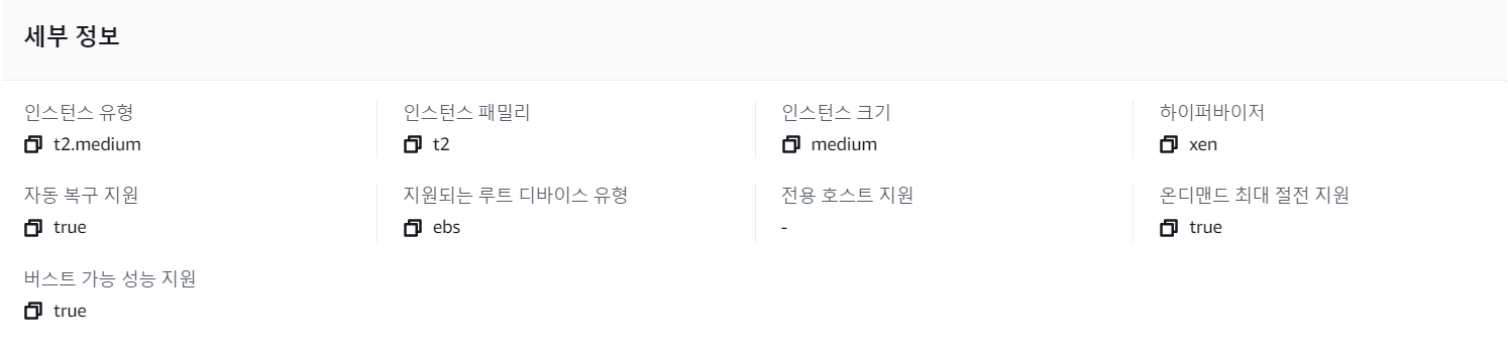
\includegraphics[width=1\textwidth]{img/t2_medium_specific.png}
\caption{t2.medium 인스턴스의 자세한 사양을 나타내는 그림입니다. 이는 인스턴스 타입, vCPU 수, 메모리 용량 등을 포함하여 AWS EC2에서 t2.medium 인스턴스 제공과 관련된 핵심 하드웨어 특성에 대한 정보를 제공합니다.}
\label{fig:t2_medium_specific}
\end{figure}

이 인스턴스는 효율적인 비용으로 안정적인 성능을 제공하며, 중소규모의 웹 애플리케이션 호스팅에 적합합니다.

\begin{figure}[H]
\centering
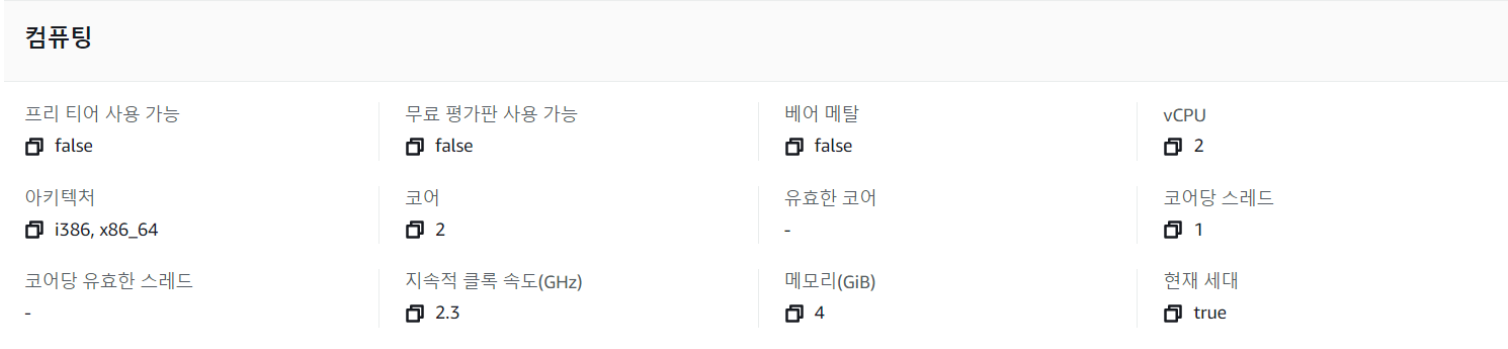
\includegraphics[width=1\textwidth]{img/t2_medium_performance.png}
\caption{이 그림은 t2.medium 인스턴스의 성능 능력을 보여주며, 컴퓨트 성능 벤치마크와 메모리 읽기/쓰기 속도를 포함한 다양한 성능 지표를 포함합니다.}
\label{fig:t2_medium_performance}
\end{figure}

성능 지표는 애플리케이션의 요구 사항에 맞추어 인스턴스를 선택하는 데 중요한 정보를 제공합니다.

\begin{figure}[H]
\centering
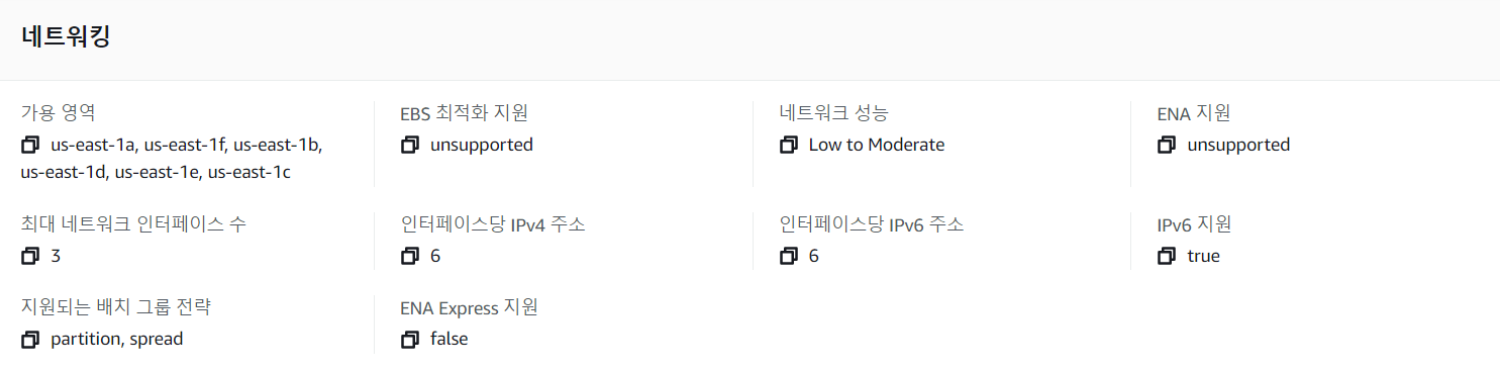
\includegraphics[width=1\textwidth]{img/t2_medium_networking.png}
\caption{이 그림은 t2.medium 인스턴스의 네트워킹 능력에 대한 정보를 보여줍니다. 네트워크 대역폭, 데이터 전송률, 지연 시간 등이 포함됩니다.}
\label{fig:t2_medium_networking}
\end{figure}

애플리케이션이 네트워크 집약적인 작업을 수행하는 경우, 이와 같은 네트워킹 성능은 매우 중요한 요소가 됩니다.

\begin{figure}[H]
\centering
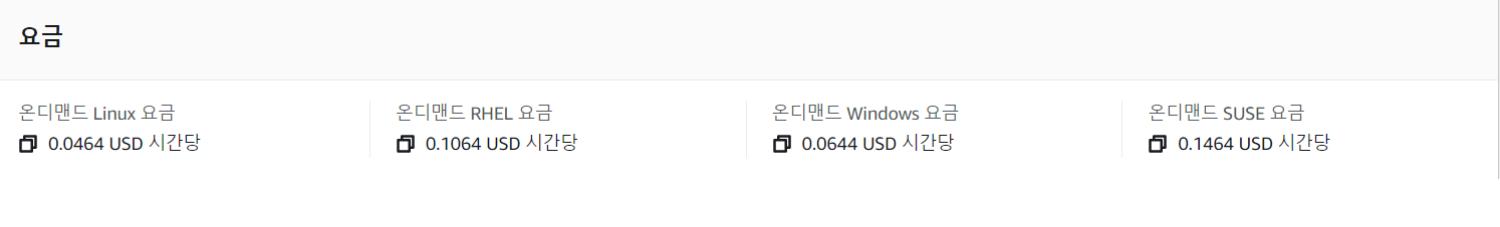
\includegraphics[width=1\textwidth]{img/t2_medium_pricing.png}
\caption{이 그림은 t2.medium 인스턴스에 대한 가격 정보를 제공합니다. 이는 시간당 비용과 필요에 따라 발생할 수 있는 추가 요금을 포함합니다.}
\label{fig:t2_medium_pricing}
\end{figure}

비용 효율성은 클라우드 서비스를 선택할 때 중요한 고려 사항입니다. 위 그림은 사용자가 비용을 예측하고 예산을 계획하는 데 도움이 됩니다.


\subsection{Software Interfaces}

node (v20.9.0), npm (v 10.2.1)과 Chat-GPT 4.0 사용해 개발되었다. 사용자는 Chrome (v45), Edge (v12), Firefox (v34) 이상의 버전을 가진 Web browser로 접속해야 한다.

\subsection{Communication Interfaces}

SKKUPPT 웹서비스의 커뮤니케이션 인터페이스는 사용자가 슬라이드를 효과적으로 제작할 수 있도록 설계된, 중요한 사용자 경험 요소이다. 본 섹션에서는 사용자가 웹 기반 인터페이스를 통해 과제 발표 슬라이드를 어떻게 제작하는지에 대한 과정을 세밀하게 설명한다.

\paragraph{정보 입력 단계}
사용자는 웹 페이지의 입력 폼을 통해 자신의 발표에 필요한 정보를 제공한다. 입력해야 할 정보는 다음과 같다:

발표 주제
발표의 목적
상세 내용
청중의 특성
예상 발표 시간
\paragraph{정보 검증 및 요청 단계}
제출된 정보는 먼저 검증 과정을 거친다. 이 과정에서 입력 정보가 충분하지 않거나 명확하지 않은 경우, 웹사이트는 사용자에게 빠진 정보의 제공 또는 기존 정보의 세부적인 개선을 요청한다. 사용자에게 피드백을 제공하는 방식은 명확하고 이해하기 쉬운 메시지를 통해 이루어져야 하며, 추가 정보 입력을 용이하게 하는 인터페이스가 마련되어야 한다.

\paragraph{프롬프트 생성 및 전송 단계}
사용자가 필요한 모든 정보를 입력하면, 웹사이트 내부 알고리즘이 이를 바탕으로 구체적인 프롬프트를 생성한다. 이 프롬프트는 사용자에게 보여지지 않고, 대형 언어 모델인 GPT(예: Chat-GPT)에 직접 전송된다.

\paragraph{GPT 응답 및 사용자 피드백 단계}
GPT는 전송된 프롬프트를 분석하여 적절한 답변을 생성한다. 생성된 답변은 사용자에게 전달되고, 사용자는 이를 토대로 슬라이드를 구성하거나, 추가적인 정보를 요구하며 피드백을 줄 수 있다. 사용자의 피드백은 웹사이트의 개선과 더욱 정확한 프롬프트 생성에 기여한다.

\paragraph{네트워크 연결 요구사항}
이 모든 과정은 사용자의 컴퓨터가 인터넷에 연결되어 있어야 가능하다. 네트워크 연결은 안정적이어야 하며, 사용자가 질의를 보내고 답변을 받아 볼 수 있도록 서버와의 신속한 데이터 교환을 보장해야 한다.

\paragraph{가독성과 사용자 경험}
이 과정의 설명은 사용자 가이드라인, FAQ 섹션, 혹은 인터랙티브 튜토리얼 등을 통해 제공되어야 하며, 사용자에게 친숙한 언어와 명확한 지시를 사용하여 가독성을 극대화해야 한다. 또한, 웹 인터페이스는 직관적이고 사용하기 쉬워야 하며, 사용자가 요구사항을 이해하고 필요한 조치를 취하기 위한 명확한 지침을 제공해야 한다.

이렇게 세부적으로 설명된 커뮤니케이션 인터페이스는 사용자가 웹서비스를 이해하고 원활하게 사용할 수 있도록 돕는 데 필수적이며, 이는 사용자 만족도를 높이고 웹 서비스의 전반적인 효율성을 향상시키는 역할을 한다.
\section{System Features}

\subsection{User Authentication}

\subsubsection{Description and Priority}
본 시스템은 사용자가 웹페이지에 접속하여 로그인 정보를 입력할 때, 이를 데이터베이스의 정보와 신속하고 안전하게 비교하여 사용자의 신원을 확인하는 기능을 보유하고 있다. 이 기능은 시스템 보안의 첫 번째 관문으로서의 역할을 수행하며, 따라서 매우 높은 우선 순위를 갖는다. 본 기능의 중요도는 매우 높아 10점 만점에 8-9점을 할당받았다.

\subsubsection{Stimulus/Response Sequences}
\begin{itemize}
  \item 사용자가 웹 인터페이스를 통해 로그인 정보(사용자 이름과 비밀번호)를 입력한다.
  \item 시스템은 보안을 유지하면서 신속하게 입력된 데이터를 데이터베이스의 정보와 대조한다.
  \item 만약 정보가 일치하면, 시스템은 사용자에게 접근 권한을 부여하고 메인 페이지로 리다이렉트한다.
  \item 정보가 일치하지 않을 경우, 사용자에게 안전한 방식으로 오류 메시지를 표시하고, 다시 시도할 수 있는 옵션을 제공한다.
\end{itemize}

\subsubsection{Functional Requirements}
\begin{itemize}
  \item REQ-1: 시스템은 사용자의 로그인 정보를 실시간으로 처리하고, 데이터베이스와의 비교를 통해 인증 절차를 완료해야 한다.
  \item REQ-2: 시스템은 인증 과정에서 발생할 수 있는 보안 문제를 방지하기 위한 적절한 암호화 및 보안 메커니즘을 구현해야 한다.
  \item REQ-3: 시스템은 인증에 실패한 경우, 사용자에게 명확하고 이해하기 쉬운 방식으로 피드백을 제공해야 한다.
\end{itemize}

\subsection{Service Selection}

\subsubsection{Description and Priority}
사용자가 성공적으로 로그인을 마치면, pptmaker, 이미지 편집기, 텍스트 에디터 등 다양한 서비스를 포함한 서비스 선택 화면이 표시된다. 사용자는 이 화면을 통해 필요한 서비스를 선택하고 해당 기능을 이용할 수 있다. 이 기능은 사용자 경험에 중요한 영향을 미치지만, 시스템의 핵심 기능과 비교했을 때 우선 순위는 다소 낮은 편이다. 따라서 이 기능의 중요도는 1-2점으로 설정되었다.

\subsubsection{Stimulus/Response Sequences}
\begin{itemize}
  \item 사용자가 로그인 과정을 성공적으로 완료한다.
  \item 시스템은 사용자에게 서비스 선택을 위한 인터페이스를 제공한다.
  \item 사용자가 특정 서비스를 선택하면, 시스템은 사용자가 접근하고자 하는 서비스로 리다이렉트한다.
  \item 사용자는 선택한 서비스의 기능을 사용하여 필요한 작업을 수행할 수 있다.
\end{itemize}

서비스 선택 과정의 시나리오는 그림 \ref{fig:computer_engineering}에서 시각적으로 확인할 수 있다.

\begin{figure}[H]
\centering
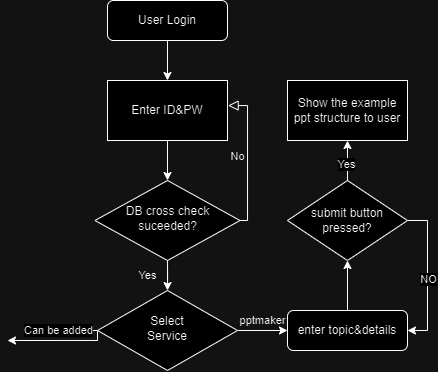
\includegraphics[width=0.7\textwidth]{img/computer_engineering.drawio.png}
\caption{서비스 선택 사용자 시나리오}
\label{fig:computer_engineering}
\end{figure}

\subsubsection{Functional Requirements}
\begin{itemize}
  \item REQ-1: 시스템은 사용자가 선택 가능한 다양한 서비스 목록을 제공해야 한다.
  \item REQ-2: 시스템은 사용자가 선택한 서비스에 따라 적절한 서비스 화면으로 안내해야 한다.
  \item REQ-3: 시스템은 서비스 간 전환과 관련된 사용자의 경험을 최적화해야 한다.
\end{itemize}


\subsection{PPT Maker}

\subsubsection{Description and Priority}
이 기능은 사용자가 주제(topic)와 세부 내용(details)을 입력하면, 시스템이 이를 GPT와 같은 고급 인공 지능 알고리즘에 전송하고, 그 결과를 사용자에게 제시하는 기능을 말한다. 특히, 사용자가 입력한 데이터를 기반으로 GPT는 관련된 PPT 콘텐츠를 생성하고 이를 사용자에게 반환한다. 이 기능의 중요도는 시스템의 다른 기능들과 균형을 이루기 위해 중간 수준인 5-6점으로 설정되었다.

\begin{figure}[H]
\centering
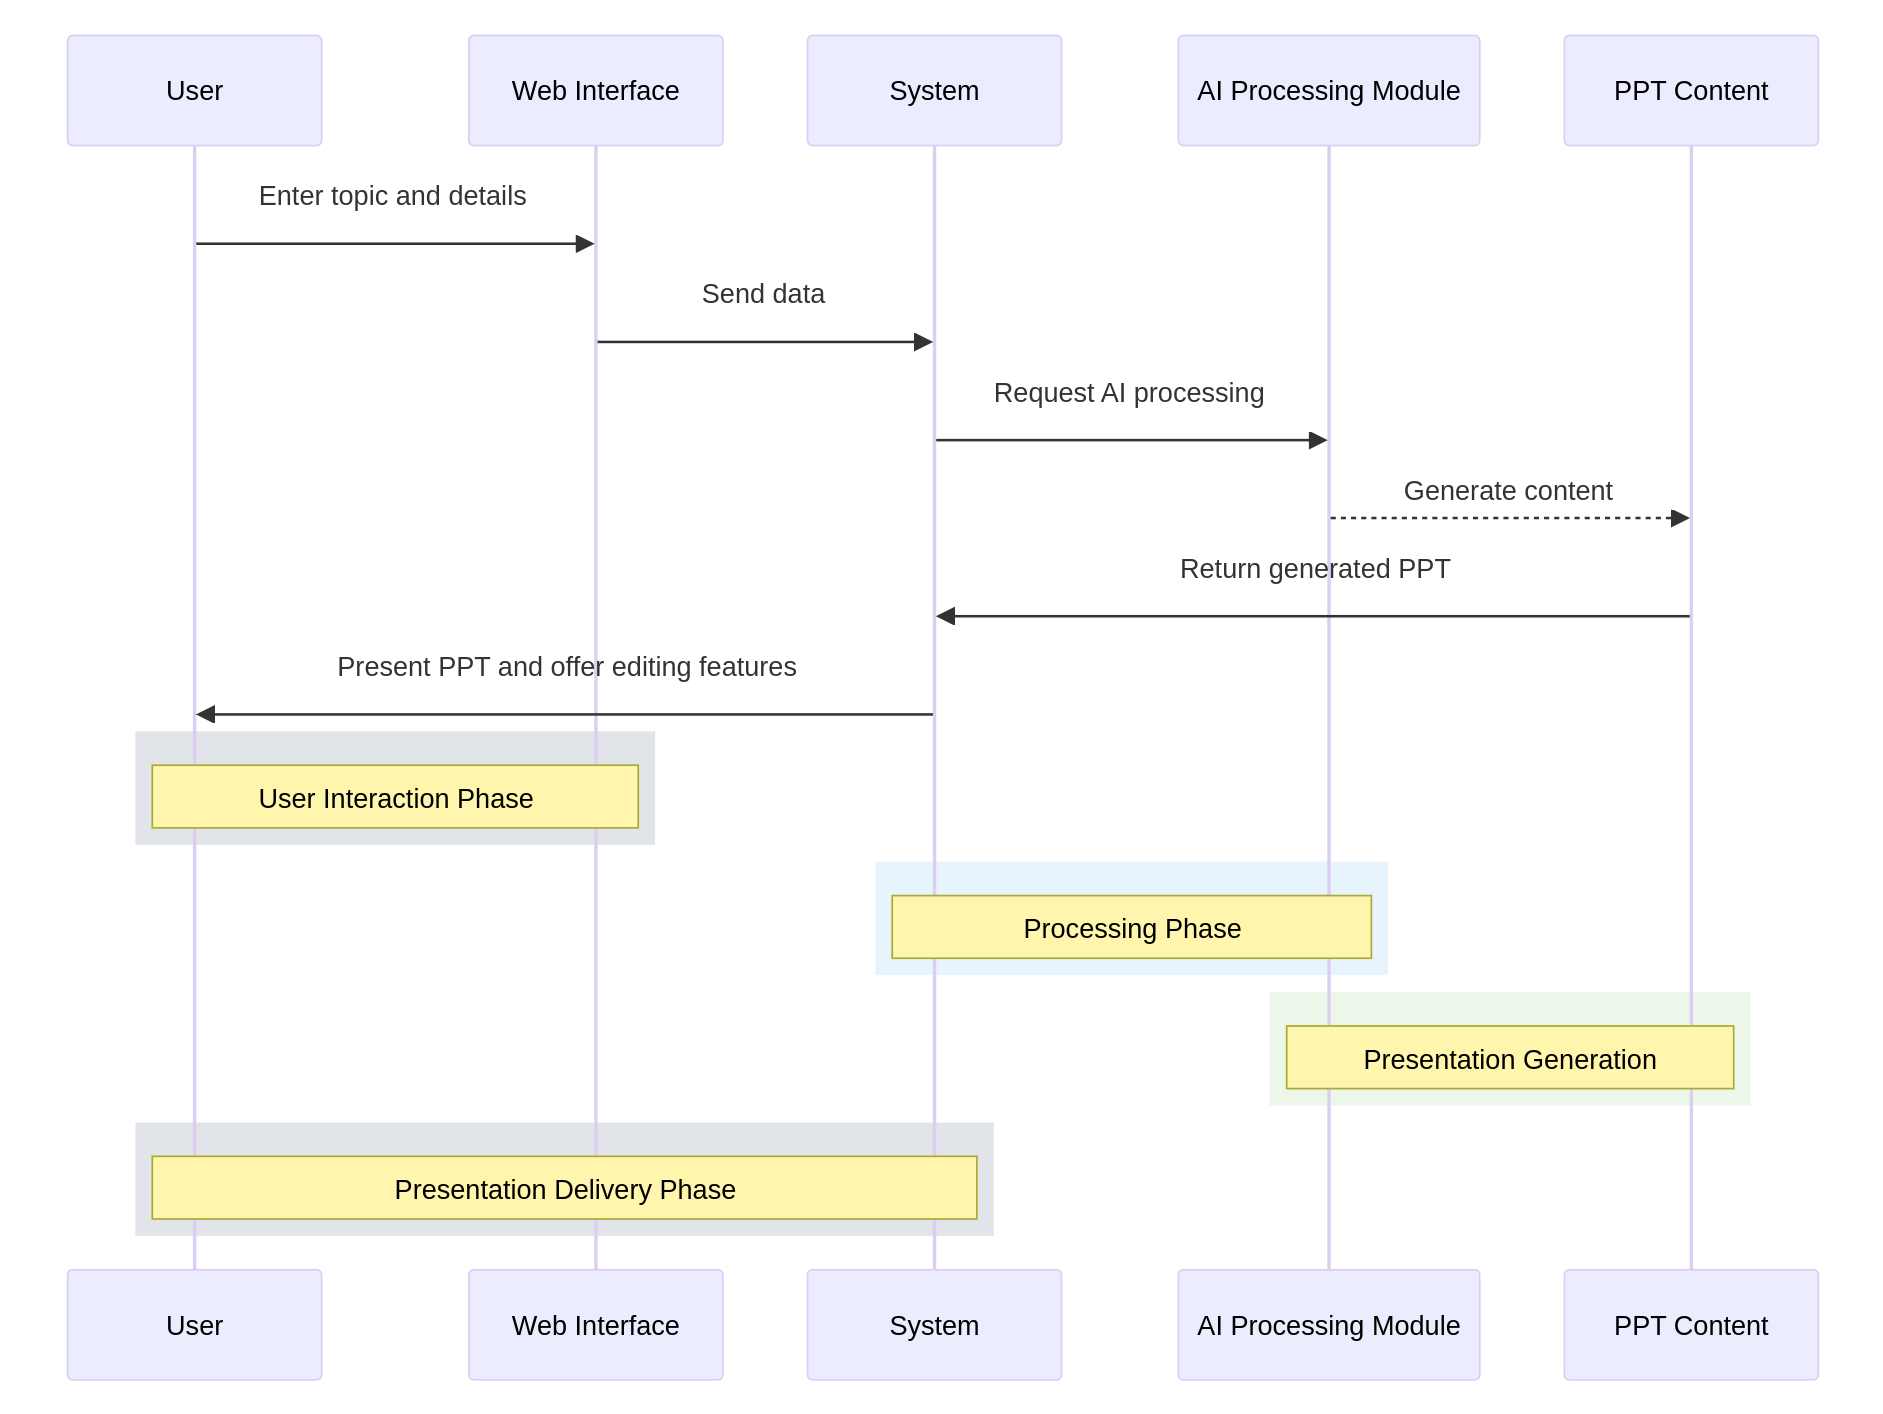
\includegraphics[width=0.9\textwidth]{img/ppt_maker.png}
\caption{PPT Maker Feature Flow}
\end{figure}

\subsubsection{Stimulus/Response Sequences}
\begin{itemize}
  \item 사용자가 주제와 세부 내용을 웹 인터페이스를 통해 입력한다.
  \item 시스템은 입력된 데이터를 AI 처리 모듈로 전송하고, 처리를 요청한다.
  \item AI 모듈은 요청받은 데이터를 기반으로 PPT 콘텐츠를 생성하고, 이를 시스템으로 반환한다.
  \item 시스템은 생성된 PPT 콘텐츠를 사용자에게 제시하고, 필요에 따라 편집 기능을 제공한다.
\end{itemize}

\subsubsection{Functional Requirements}
\begin{itemize}
  \item REQ-1: 시스템은 사용자의 입력(주제와 세부 내용)을 정확히 파악하고 처리할 수 있어야 한다.
  \item REQ-2: 시스템은 사용자의 입력을 바탕으로 AI에 PPT 콘텐츠 생성을 요청하고, 결과를 받을 수 있어야 한다.
  \item REQ-3: 시스템은 생성된 PPT 콘텐츠를 사용자에게 효과적으로 제시하고, 사용자가 원할 경우 추가 편집이 가능하도록 지원해야 한다.
\end{itemize}





\section{Non-Functional Requirements}

본 단락에서는 웹 애플리케이션의 비기능적 요구사항을 명세합니다. 비기능적 요구사항은 시스템의 성능, 안전성, 보안성, 품질 등을 기술하며, 이를 충족시키기 위한 제약 조건을 명시합니다. 이러한 비기능적 요구사항은 기능적 요구사항과는 다른 관점에서 사용자의 만족도를 높이고, 웹 애플리케이션의 안정성을 보장하는 데 중요한 역할을 합니다.

\subsection{Performance Requirements}

본 소프트웨어는 고성능을 목표로 하며, 다양한 성능 요구사항을 충족시킬 수 있도록 제작되었습니다.

\begin{itemize}
    \item \textbf{응답시간:} 사용자의 슬라이드 제작 요청이 서버에 도달한 후, 서버는 최대 5초 내로 사용자에게 응답을 반환해야 합니다. 이는 이용자의 대기시간을 감소시켜 결과적으로 사용자 경험(UX)을 증가시킬 것입니다.
    
    \item \textbf{동시사용자 처리능력:} 본 웹 애플리케이션은 최소한 10000명의 동시 접속 사용자를 처리할 수 있어야 합니다. 이는 서버의 확장성과 부하 분산 기능을 통해 이루어져야 합니다.
    
    \item \textbf{슬라이드 생성 속도:} AI API는 사용자의 입력 데이터와 템플릿을 기반으로 하여, 1분당 최소 20장의 슬라이드를 생성할 수 있어야 합니다.
    
    \item \textbf{데이터 전송 속도:} 사용자가 요청한 슬라이드 파일은 높은 품질로 빠르게 전송되어야 하며, 이는 네트워크 지연과 데이터 손실을 최소화하는 기술을 사용하여 달성될 수 있습니다.
    
    \item \textbf{자원 사용 효율성:} 웹 애플리케이션은 서버와 클라이언트 측 모두에서 자원을 효율적으로 사용해야 합니다. 메모리 누수 및 CPU 과부하 없이 안정적인 성능을 지속적으로 제공해야 합니다.
    
    \item \textbf{확장성:} 시스템은 사용자 수가 증가함에 따라 선형적으로 확장될 수 있어야 하며, 이를 위해 클라우드 기반 인프라를 활용하여 자동 확장 기능을 구현해야 합니다.
    
    \item \textbf{장애 복구 시간:} 만약 시스템에 장애가 발생한 경우, 최대한 빠르게 복구되어야 하며, 목표 복구 시간(RTO)은 5분 이내로 설정됩니다.
\end{itemize}

이러한 성능 요구사항들은 웹 애플리케이션의 안정성과 사용자 만족도를 높이기 위해 필요하며, 지속적인 모니터링과 테스트를 통해 이를 만족하는지 확인해야 합니다.

\subsection{Safety Requirements}

사용자의 안전과 데이터 보호를 최우선으로 하는 여러 안전 요구사항을 충족해야 합니다. 안전 요구사항의 주요 목표는 사용자 데이터의 보호와 서비스의 안정적인 제공을 통해 사용자의 신뢰를 얻는 것입니다.

\begin{itemize}
    \item \textbf{개인 정보 보호:} 사용자의 개인 정보를 수집, 저장, 처리할 때, GDPR(General Data Protection Regulation)과 같은 국제적인 데이터 보호 규정을 준수해야 합니다. 사용자의 명시적인 동의 없이 개인 정보를 수집하거나 제 3자와 공유하지 않아야 합니다.
    
    \item \textbf{데이터 암호화:} 사용자의 개인 정보와 슬라이드 데이터는 전송 중과 저장 시 모두 암호화되어야 합니다. HTTPS를 사용하여 웹 트래픽을 암호화하고, 데이터베이스에 저장된 정보 역시 적절한 암호화 기술을 사용하여 보호해야 합니다.
    
    \item \textbf{에러 핸들링과 예외 관리:} 예기치 못한 입력이나 시스템 오류가 발생해도 안전하게 처리할 수 있는 방안을 갖추어야 합니다. 시스템의 안정성을 해치지 않는 선에서 사용자에게 명확한 에러 메시지를 제공해야 합니다.
    
    \item \textbf{백업과 복구:} 사용자 데이터와 서비스 관련 데이터는 정기적으로 백업되어야 하며, 장애 발생 시 빠르게 복구할 수 있도록 해야 합니다. 이를 위해 데이터 복구 전략과 백업 주기 등을 명확하게 정의해야 합니다.
    
    \item \textbf{시스템 접근 제어:} 웹 애플리케이션과 관련 인프라에 대한 접근은 엄격하게 제어되어야 하며, 필요한 권한만을 적절한 수준에서 부여해야 합니다. 무단 접근이나 데이터 변조를 방지하기 위한 인증 및 권한 관리 시스템을 구축해야 합니다.
\end{itemize}

\subsection{Security Requirements}
\begin{itemize}
    \item \textbf{데이터 전송의 암호화:} HTTPS를 사용하여 사용자의 민감한 정보를 암호화하여 전송해야 합니다. 이는 중간자 공격을 방지하고 데이터의 기밀성을 보장합니다.
    
    \item \textbf{정기적인 보안 업데이트 및 패치:} 보안 취약점을 신속하게 해결하기 위해 정기적으로 소프트웨어 업데이트와 패치를 수행해야 합니다.

    \item \textbf{인증 및 권한 관리:} 사용자의 신원을 확인하는 강력한 인증 과정을 거치고, 적절한 권한을 부여해야 합니다.

    \item \textbf{입력 데이터 검증:} 사용자로부터 입력 받는 모든 데이터는 서버 측에서 검증되어야 하며, 공격으로부터 시스템을 보호해야 합니다.

    \item \textbf{로그 및 모니터링:} 사용자의 접근 로그와 시스템의 작동 로그를 지속적으로 기록하고 모니터링해야 합니다.

    \item \textbf{비상계획 및 인시던트 응답:} 보안 인시던트 발생 시 신속하게 대응할 수 있는 프로세스와 계획을 갖추어야 합니다.
\end{itemize}

\subsection{Software Quality Attributes}
\begin{itemize}
    \item \textbf{Usability:} 사용자 친화적인 인터페이스를 제공해야 합니다.
    
    \item \textbf{Reliability:} 정확하고 일관된 결과를 제공해야 합니다.

    \item \textbf{Performance:} 사용자의 요청에 빠르게 응답하고, 트래픽을 유연하게 처리해야 합니다.

    \item \textbf{Scalability:} 사용자 수나 데이터 양이 증가함에 따라 쉽게 확장될 수 있어야 합니다.

    \item \textbf{Maintainability:} 코드의 가독성, 모듈화, 재사용성을 고려하여 개발되어야 합니다.

    \item \textbf{Portability:} 다양한 브라우저와 운영 체제에서도 문제 없이 실행될 수 있어야 합니다.

    \item \textbf{Security:} 사용자 데이터의 기밀성, 무결성, 가용성을 보장해야 합니다.
\end{itemize}

\subsection{Business Rules}
\begin{itemize}
    \item \textbf{데이터 소유권 및 저작권:} 사용자가 업로드하는 모든 데이터와 생성된 슬라이드는 사용자의 소유입니다.

    \item \textbf{사용자 프라이버시:} 사용자의 개인정보를 보호하며, 개인정보처리방침을 명시해야 합니다.

    \item \textbf{서비스 이용 약관:} 사용자에게 서비스 이용 약관을 제공하고, 동의 후에 서비스를 이용할 수 있어야 합니다.

    \item \textbf{결제 및 환불 정책:} 유료 서비스를 제공하는 경우, 명확한 결제 및 환불 정책을 제공해야 합니다.

    \item \textbf{서비스 가용성 및 연속성:} 지속적이고 안정적인 서비스 제공을 위해 노력해야 합니다.

    \item \textbf{법적 준수:} 해당 지역 및 국가의 법률과 규정을 준수해야 합니다.
\end{itemize}


\appendix
\section{Appendix: Analysis Models}
%\addcontentsline{toc}{section}{Appendix: Analysis Models}

시스템 아키텍처는 \cite{sommerville2015software}에 따라 UML을 통해 설명된다. 전반적인 UML 작성은 \cite{sveidqvist2021official}를 챀조하였다. 이것은 추상적인 요구사항으로, 변경 가능한 부분을 포함한다. 

\subsection{Entity-Relationship Requirements}

엔티티-관계 다이어그램(ERD)은 시스템의 데이터 모델을 나타냅니다. 이것은 사용자가 우리 시스템과 상호 작용하고 프레젠테이션을 관리하는 방법, 그리고 그들의 상호 작용이 어떻게 기록되고 API 사용이 추적되는지를 보여줍니다.

\begin{figure}[H]
\centering
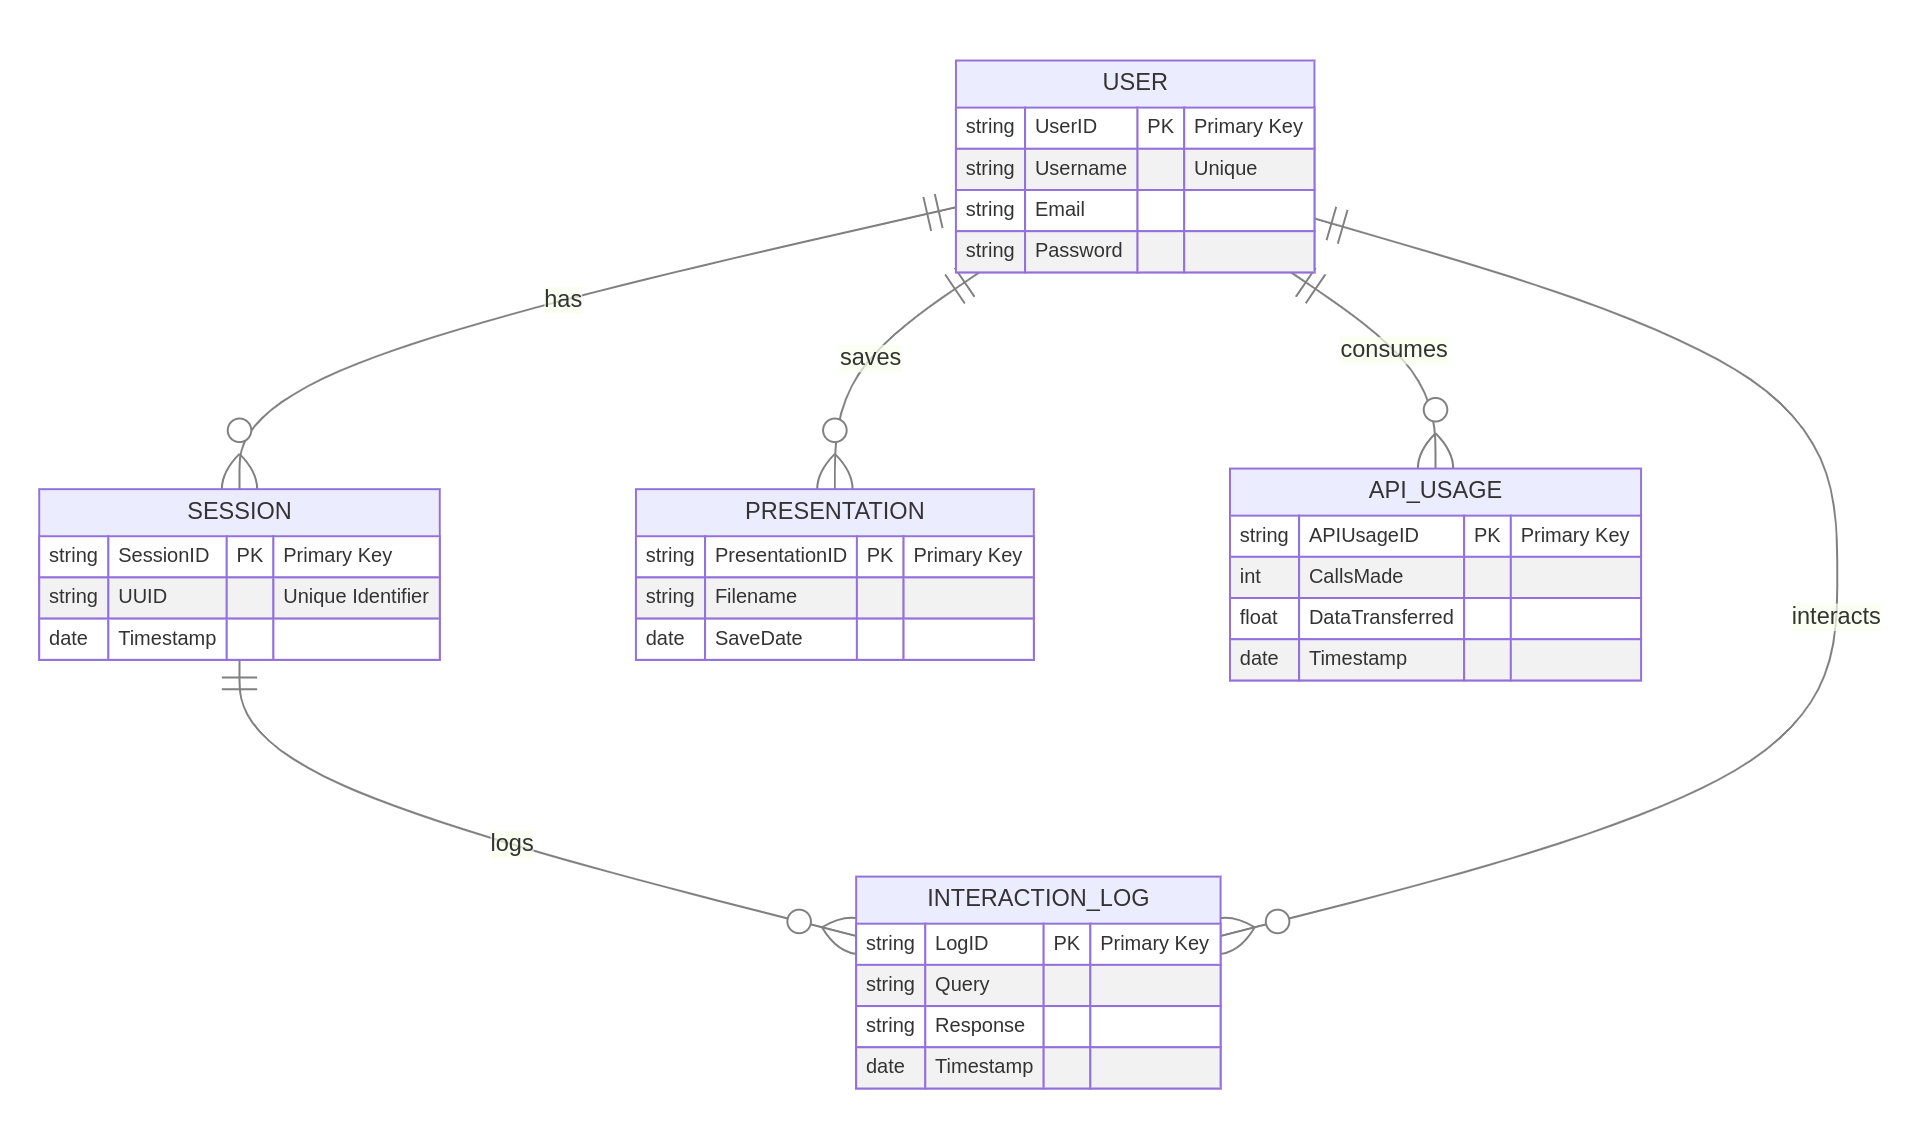
\includegraphics[width=1\textwidth]{img/er_diagram.png}
\caption{Entity-Relationship Diagram}
\label{fig:er_diagram}
\end{figure}

그림 \ref{fig:er_diagram}에 나타난 ER 다이어그램은 사용자와 그들의 로그인 세션, 저장된 파워포인트 프레젠테이션, ChatGPT API와의 상호 작용 로그, 그리고 API 사용 메트릭 간의 관계를 보여줍니다.


\subsection{Sequence Diagram}

시퀀스 다이어그램은 DNS, AWS 인스턴스, Nginx 프록시를 포함한 여러 시스템 구성 요소를 통해 브라우저 사용자와 ChatGPT API 간의 상호 작용을 보여줍니다. 그림 \ref{fig:sequence_diagram}에 묘사된 바와 같이, 사용자의 요청은 DNS Route53에 의해 해결되고, AWS 인스턴스와 Nginx 프록시를 거쳐, 마지막으로 ChatGPT API와 통신하는 Next.js 애플리케이션에 의해 처리됩니다.

\begin{figure}[H]
\centering
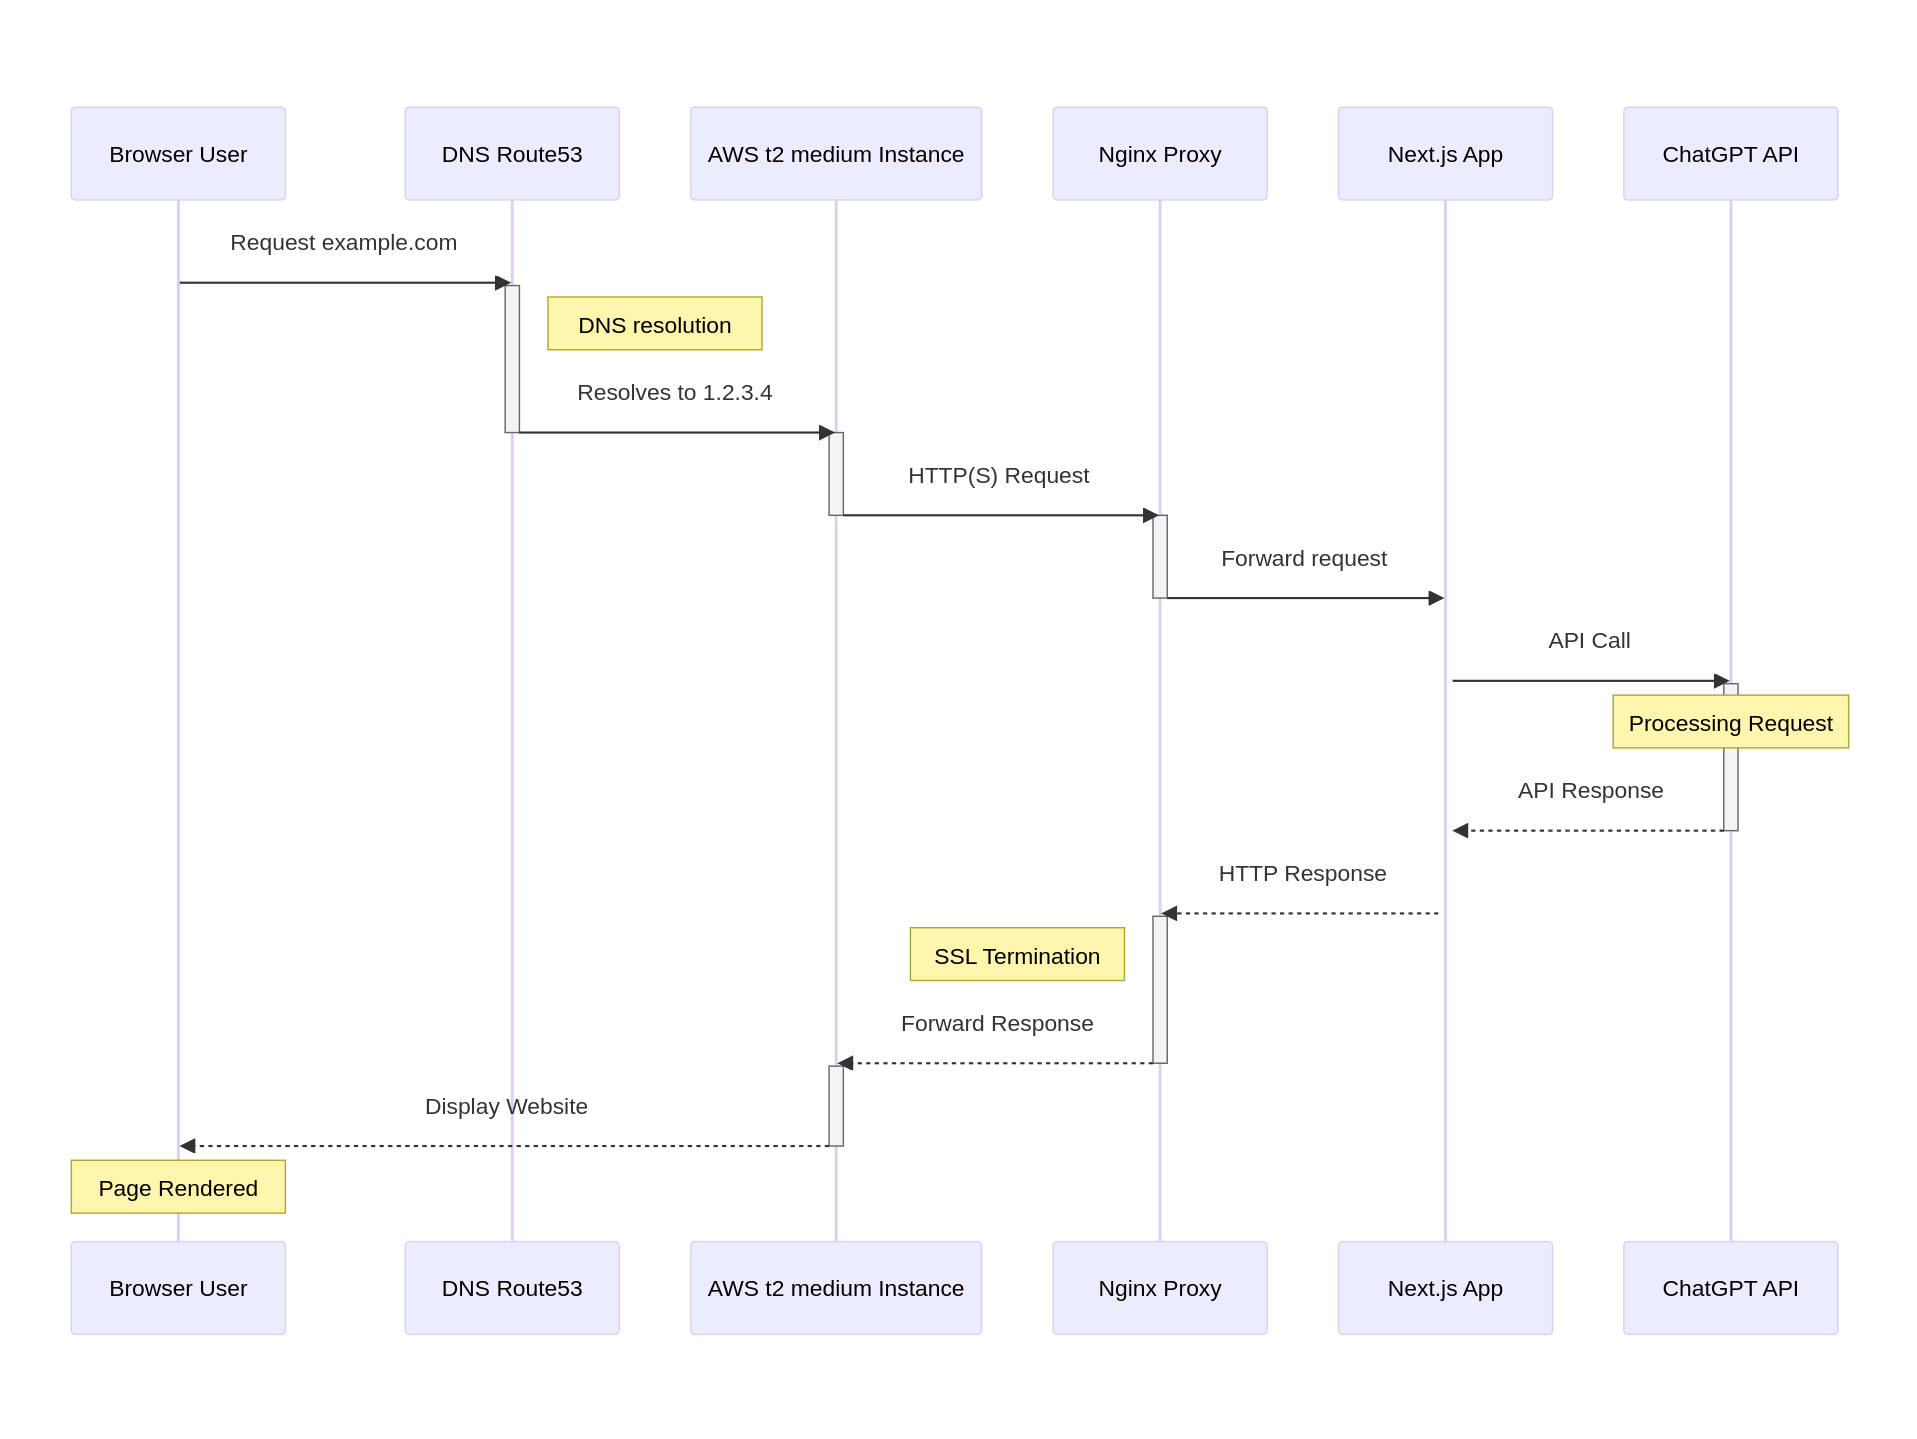
\includegraphics[width=1\textwidth]{img/sequence_diagram.png}
\caption{Sequence diagram of the interaction flow within the system.}
\label{fig:sequence_diagram}
\end{figure}

\subsection{State Diagram}

아래 상태 다이어그램은 사용자의 요청을 처리하는 여러 단계를 개략적으로 설명합니다. 시스템의 운영 상태와 전환에 대한 자세한 내용은 그림 \ref{fig:state_diagram}을 참조하십시오.

\begin{figure}[H]
\centering
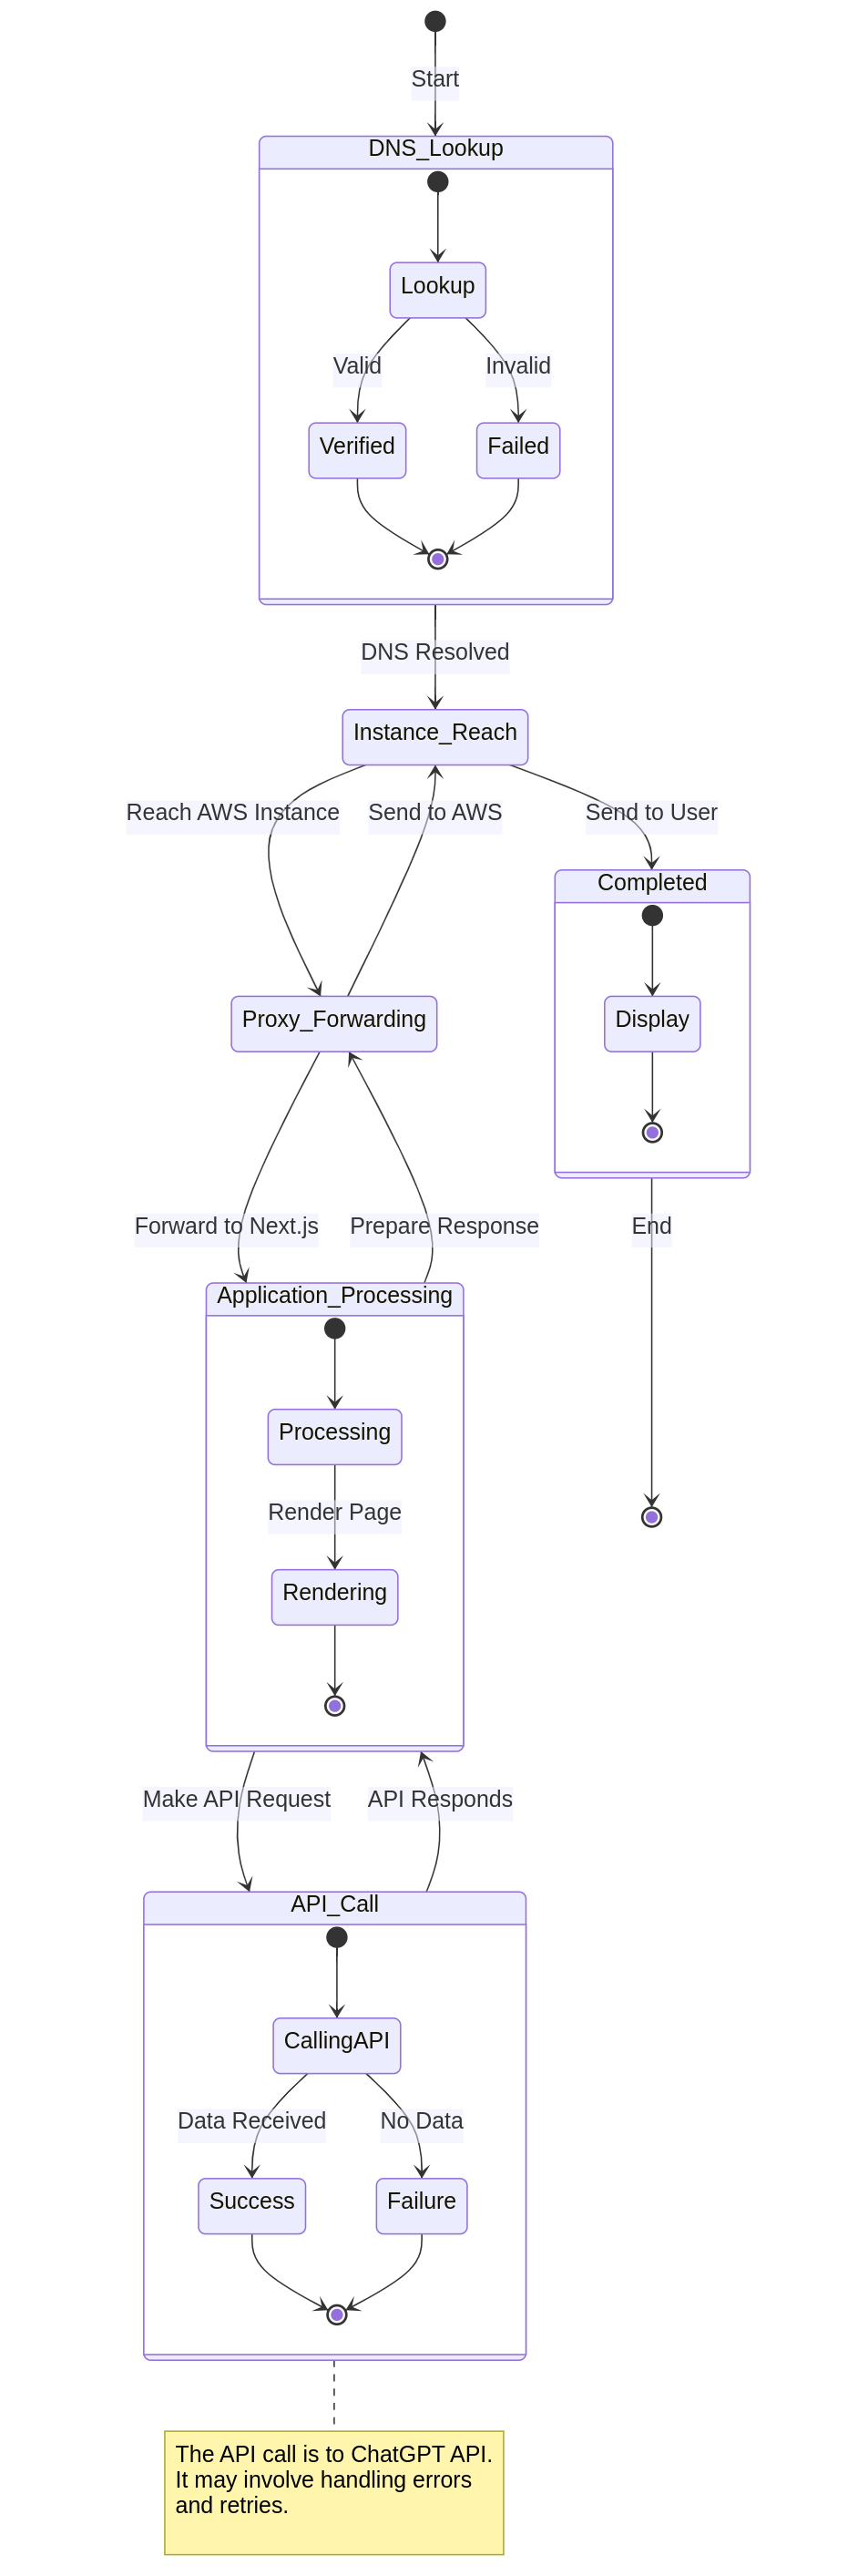
\includegraphics[width=0.5\textwidth]{img/state_diagram.png}
\caption{State diagram representing the flow of a user request through the system.}
\label{fig:state_diagram}
\end{figure}



\end{document}

